\subsection{\IFRU{Сдвиги}{Shifts}}

\IFRU{Битовые сдвиги в \CCpp реализованы при помощи операторов $\ll$ и $\gg$.}
{Bit shifts in \CCpp are implemented via $\ll$ and $\gg$ operators.}

\IFRU{Вот этот несложный пример иллюстрирует функцию, считающую количество бит-единиц во входной переменной:}
{Here is a simple example of function, calculating number of 1 bits in input variable:}

\lstinputlisting{14_bitfields/shifts.c}

\IFRU{В этом цикле, счетчик итераций \IT{i} считает от 0 до 31, а $1 \ll i$ будет от 1 до 0x80000000. 
Описывая это словами, можно сказать 
\IT{сдвинуть единицу на n бит влево}.
Т.е., в некотором смысле, выражение $1 \ll i$ последовательно выдаст все возможные позиции бит в 32-битном числе. 
Кстати, освободившийся бит справа всегда обнуляется. Макрос \TT{IS\_SET} проверяет наличие этого бита в \TT{a}.}
{In this loop, iteration count value \IT{i} counting from 0 to 31, $1 \ll i$ statement will be counting from 1 to 0x80000000. 
Describing this operation in natural language, we would say \IT{shift 1 by n bits left}.
In other words, $1 \ll i$ statement will consequently produce all possible bit positions in 32-bit number.
By the way, freed bit at right is always cleared. \TT{IS\_SET} macro is checking bit presence in \TT{a}.}

\begin{figure}[ht!]
\centering
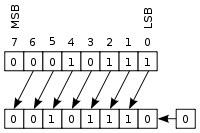
\includegraphics[scale=0.66]{14_bitfields/200px-Rotate_left_logically.png}
\caption{\IFRU{Как работает инструкция \SHL\protect\footnotemark}
{How \SHL instruction works\protect\footnotemark}}
\end{figure}

\footnotetext{\IFRU{иллюстрация взята из}{illustration taken from} wikipedia}

\IFRU{Макрос \TT{IS\_SET} на самом деле это операция логического И (\IT{AND}) 
и она возвращает ноль если бита там нет, 
либо эту же битовую маску, если бит там есть. 
В \CCpp, конструкция \TT{if()} срабатывает, если выражение внутри её не ноль, пусть хоть 123, 
поэтому все будет работать.}
{The \TT{IS\_SET} macro is in fact logical and operation (\IT{AND}) 
and it returns zero if specific bit is absent there,
or bit mask, if the bit is present.
\IT{if()} operator triggered in \CCpp if expression in it isn't zero, it might be even 123, that's why
it always working correctly.}

\IFRU{Компилируем}{Let's compile} (MSVC 2010):

\lstinputlisting[caption=MSVC 2010]{\IFRU{14_bitfields/shifts_MSVC_ru.asm}{14_bitfields/shifts_MSVC_en.asm}}

\IFRU{Вот так работает SHL (\IT{SHift Left})}{That's how SHL (\IT{SHift Left}) working}.

\IFRU{Скомпилируем то же и в}{Let's compile it in} GCC 4.4.1:

\lstinputlisting[caption=GCC 4.4.1]{14_bitfields/shifts_gcc.asm}

\IFRU{Инструкции сдвига также активно применяются при делении или умножении 
на числа-степени двойки (1, 2, 4, 8, итд).}
{Shift instructions are often used in division and multiplications by power of two numbers (1, 2, 4, 8, etc).}

\IFRU{Например:}{For example:}

\begin{lstlisting}
unsigned int f(unsigned int a)
{
	return a/4;
};
\end{lstlisting}

\IFRU{Имеем в итоге}{We got} (MSVC 2010):

\begin{lstlisting}[caption=MSVC 2010]
_a$ = 8							; size = 4
_f	PROC
	mov	eax, DWORD PTR _a$[esp-4]
	shr	eax, 2
	ret	0
_f	ENDP
\end{lstlisting}

\label{SHR}
\IFRU{Инструкция \SHR (\IT{SHift Right}) в данном примере сдвигает число на 2 бита вправо. 
При этом, освободившиеся два бита слева (т.е., самые 
старшие разряды), выставляются в нули. А самые младшие 2 бита выкидываются. 
Фактически, эти два выкинутых бита ~--- остаток от деления.}
{\SHR (\IT{SHift Right}) instruction in this example is shifting a number by 2 bits right.
Two freed bits at left (e.g., two most significant bits) are set to zero.
Two least significant bits are dropped.
In fact, these two dropped bits ~--- division operation remainder.}

\IFRU{Инструкция \SHR работает так же как и \SHL, только в другую сторону.}
{\SHR instruction works just like as \SHL but in other direction.}

\begin{figure}[ht!]
\centering
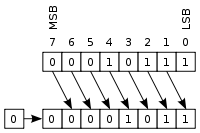
\includegraphics[scale=0.66]{14_bitfields/200px-Rotate_right_logically.png}
\caption{\IFRU{Как работает инструкция \SHR\protect\footnotemark}
{How \SHR instruction works\protect\footnotemark}}
\end{figure}

\footnotetext{\IFRU{иллюстрация взята из}{illustration taken from} wikipedia}

\IFRU{Для того, чтобы это проще понять, представьте себе десятичную систему счисления и число 23. 
23 можно разделить на 10 просто выкинув последний разряд (3 ~--- это остаток от деления). 
После этой операции останется 2 как частное
\footnote{результат деления}.}
{It can be easily understood if to imagine decimal numeral system and number 23.
23 can be easily divided by 10 just by dropping last digit (3 ~--- is division remainder). 
2 is leaving after operation as a quotient
\footnote{division result}.}

\IFRU{Так и с умножением. Умножить на 4 это просто сдвинуть число на 2 бита влево, 
вставив 2 нулевых бита справа (как два самых младших бита). 
Это как умножить 3 на 100 ~--- нужно просто дописать два нуля справа.}
{The same story about multiplication. Multiplication by 4 is just shifting the number to the left by 2 bits,
inserting 2 zero bits at right (as the last two bits).
It's just like to multiply 3 by 100 ~--- we need just to add two zeroes at the right.}
